\section{The SwipeVR Text Entry Technique}


This design is a special case of relative finger tracking in that it uses inspiration in Swype. 
The user draws a trail which is then translated to a series of taps on the 6 keys tap keyboard through finding the inflection points on the user's finger movement path.
We describe a specialized keyboard for text entry that maps six rows of a standard keyboard onto a virtual keyboard, shown in Figure~\ref{fig:swipeVRLayout}.
Different words are encoded via modifier keys and multi-swipe input with the thumb.
Use of the keyboard also relies on lexicon-based disambiguation.

\subsection{Slow and Fast Keyboard}
\subsection{Gesture Detection}
A special case of relative finger tracking is the 6 Keys Swype keyboard design.
This keyboard design resembles the use of Swype keyboard on Android.
In such a case, finger swipe data needs to be translated to a sequence of numbers to denote the chosen letters
We implement this functionality by finding the inflection points along the path (see Figure~\ref{fig:position}).
After a few experimental trials, we realized that as the user changes direction of his finger movement, the speed of his finger movement decreases (see Figure~\ref{fig:acceleration}).
Combining actual directional changes of the swipe trail, we are able to identify the inflection points. 

\subsection{Special Interactions}



Interaction with keyboards with relative finger tracking requires extra layers of complication by the nature of the swiping motion.
Special means of interaction such as space and delete becomes a none trivial task for the user would need to drag the virtual cursor to a designated location.
However, this form of interaction is against the motive of the finger tracking motion, which is to simplify users' interaction with the keyboard.
Thus, we designate new forms of interaction to help users use space and delete utility quickly.
Presses and hold on the trigger as shown in Figure~\ref{fig:trigger} to show a list of special keys, as shown in Figure~\ref{fig:specialCharacters}.


\subsection{Deterministic Inputs}
Measure for 0 acceleration as shown in Figure~\ref{fig:acceleration}.

\subsubsection{Delete}
For delete, users can double tap the mobile phone screen.

\subsubsection{Space}
To insert a space, the user clicks the trigger button on the bottom side of the controller, as shown in Figure~\ref{fig:trigger}. 
We experimented with automatically inserting a space after a certain timeout periods between 150 and 500ms.  However, we found that users prefered to have the control of when to insert the space themselves.




\subsubsection{Word option}
Long swipe


\begin{figure}
  \centering

  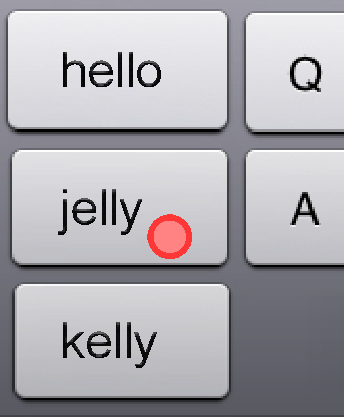
\includegraphics[width=.3\columnwidth]{figures/multiword}
  
  \caption{The Bayesian word recommender infers the most probable words with the same representation as the entered batched keys. In the above example, \textit{hello}, \textit{jelly}, and \textit{kelly} have the same representation, Key 5, 1, 5, 5, then 4. The algorithm uses 2-gram and 3-gram data from Google, part of speech frequency for English dictionary, word frequency for the entire English language, and produces a prediction score. The word with highest prediction score is the default output.  The user can \textit{long-swipe} to select alternate choices.}
  ~\label{fig:multiword}
\end{figure}


Another form of special interaction worth mentioning is choosing word options.
With batched keys, the word users input may contain uncertainty - multiple words with the same representation. See Figure~\ref{fig:multiword}.

Although the word recommender algorithm will produce the most likely word, it is not guaranteed such word is the choice of the users.
Thus, we enable users to choose among the next few most probable options.
The users simply drag towards the direction of the displayed option to choose the alternatives.

\subsection{Bayesian Word Recommender}
The Bayesian word recommender aims to infer the most probable words with the same representation in the same configuration of batched keys.
For instance, in 6 keys designs, word ``hello" and ``jelly" has the same representation ``51554".
This recommender algorithm use 2-gram and 3-gram data from Google Books Ngram Viewer\footnote{http://storage.googleapis.com/books/ngrams/books/datasetsv2.html}, part of speech frequency for English dictionary, individual word frequency for the entire English language, and produces a prediction score.
The word with highest prediction score will be selected as the most probable word.

\subsection{Implementation}
SwipeVR consists of three components: software for the controller , software for the virtual reality display, and a back end software.
The controller software (Android or HTC Vive) collects the finger movement from the users and relay the data to back end server.
The data relayed varies for different input methods.
For relative finger tracking, an unscaled change vector is emitted for every unit time interval to show the finger movement on screen, whereas absolute finger tracking, a pair of scaled coordinates are sent to show the position of the touch on the screen.
For designs with batched keys, a number indicating which key is selected is also emitted, whereas designs with 26 individual keys emits no additional information.
Selection of letter is determined based on the position of the cursor in virtual reality. (see Figure~\ref{fig:systemScreenshot})(see Figure~\ref{fig:systemFlowchart})

The back end server collects these finger movement data described above.
If the design uses batched keys, the inputted number sequence will go through a Bayesian algorithm that determines the most probable word with the same batched key combinations. The produced word is then sent to the virtual reality environment for display.
On the other hand, if no batched keys are used, finger position data will be directly sent to the virtual reality environment for display.



\begin{figure}
  \centering


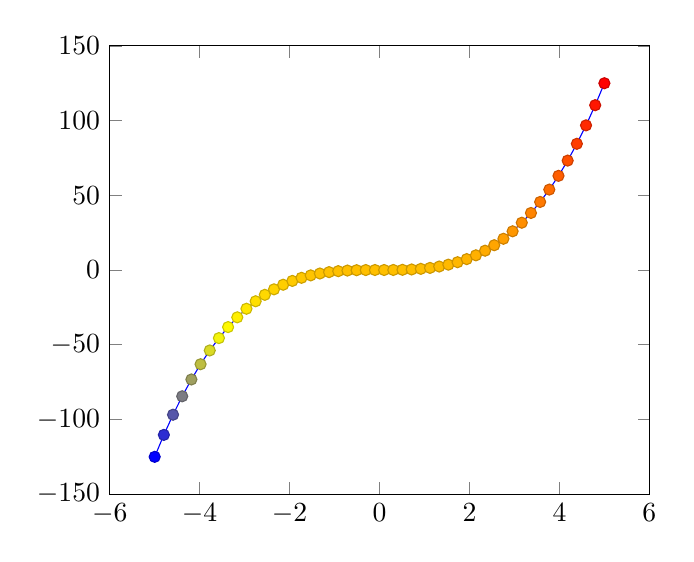
\begin{tikzpicture}
\begin{axis}
\addplot+[scatter,
samples=50,scatter src=y]
{x^3};
\end{axis}
\end{tikzpicture}
	\caption{Gesture detection graph with acceleration}~\label{fig:acceleration}
\end{figure}

\begin{figure}
\centering
  \begin{tikzpicture}
  \begin{axis}[
    xlabel=$x$,
    ylabel=$\sin(x)$
  ]
    \addplot gnuplot[id=sin]{sin(x)}; 
  \end{axis}
\end{tikzpicture}

  
  \caption{Gesture tracking graph with position}~\label{fig:position}
\end{figure}



\subsection{Overall Structure}
The system is composed of three parts: an Android client, a backend server and a virtual environment. The Android client parses finger movement to letters. In some cases, such as Swype with 6 keys, finger movement data are processed to groups numbers by an algorithm that takes acceleration and direction change of finger to find inflection points on the path.

\subsection{Client-side}
The Android client then relays user input to the backend where the input is passed through a Bayesian model, using dictionary word frequency, part of speech frequency, and Google NGram data Such model determines the most likely word, which is sent to the virtual environment for display.

\subsection{Visual interface design}
Designing effective visual interfaces is critical to the overall usability of the system. Here we present some of the key components of used in this regard. 

\subsubsection{Feedback and output interfaces}
\subsubsection{Managing Visual Attention 1}


\begin{figure}
  \centering
  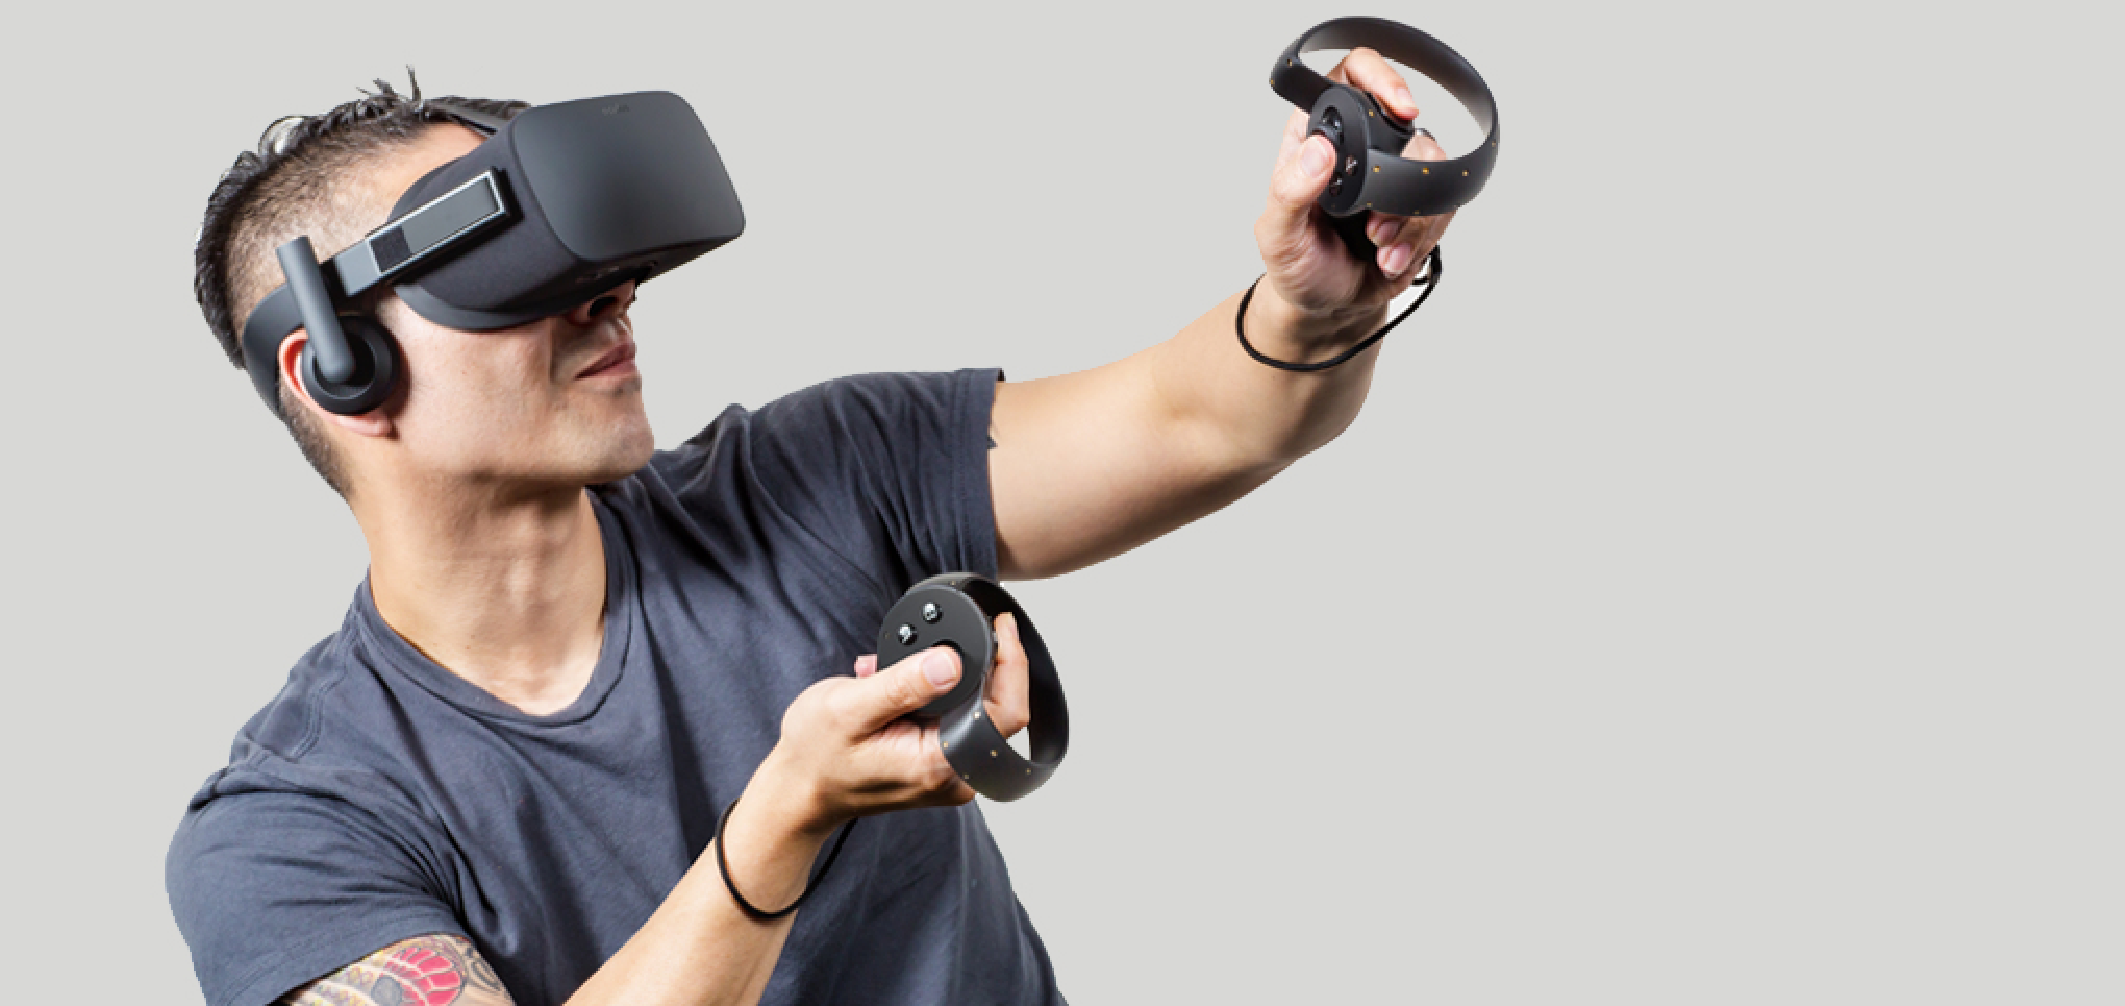
\includegraphics[width=1\columnwidth]{figures/manVR}
  \caption{User using SwipeVR.}~\label{fig:figure2}
\end{figure}


\begin{table}
  \centering
  \begin{tabular}{l r r r r}
    % \toprule
    & & \multicolumn{2}{c}{\small{\textbf{Test Conditions}}} \\
    \cmidrule(r){2-5}
    {\small\textit{Input}}
    & {\small \textit{Speech}}
    & {\small \textit{Mobile Keyboard}}
    & {\small \textit{Gaze}}
    & {\small \textit{SwipeVR}} \\
    \midrule
    Words per Minute & 152 & 52 & 9 & 49 \\
    Uncorrected Error Rate & 3\% & 3\% & 3\% & 3\% \\
    Corrected Error Rate & 3\% & 3\% & 3\% & 3\%\\
    Total Error Rate & 3\% & 3\% & 3\% & 3\%\\
    % \bottomrule
  \end{tabular}
  \caption{ Mean measures for the four input methods.}~\label{tab:tableResults}
\end{table}

\begin{figure}
\centering
\begin{tikzpicture}
\begin{axis}
\addplot+[ybar] plot coordinates
{(0,3) (1,2) (2,4) (3,1) (4,2)};
\end{axis}
\end{tikzpicture}

\caption{Words per minute as a function of language and input method.}~\label{fig:graphWPM}
\end{figure}

\begin{figure}
\centering

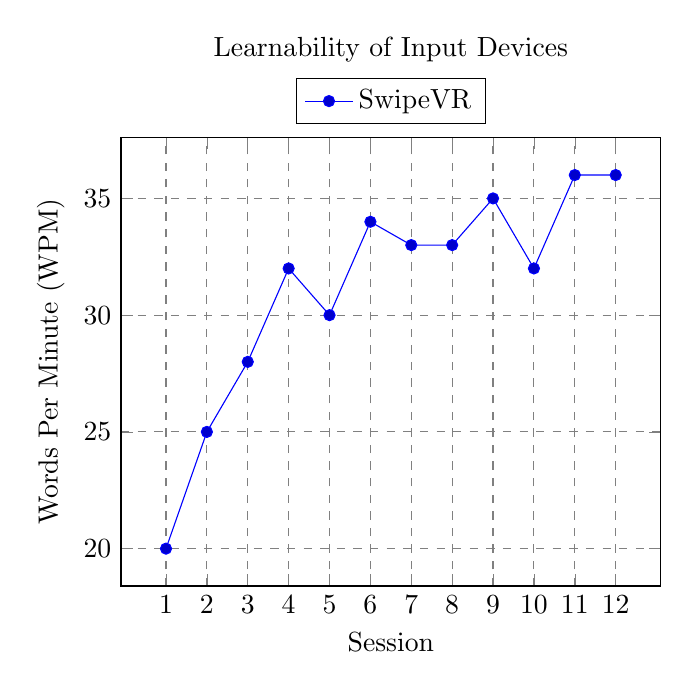
\begin{tikzpicture}
\pgfplotsset{
		every axis legend/.append style={
			at={(0.5,1.03)
		},
		anchor=south
    }
}
\pgfplotsset{grid style={dashed,gray}}
%\pgfplotsset{minor grid style={dashed,red}}
%\pgfplotsset{major grid style={dotted,green!50!black}}

\begin{axis}[
legend columns=-1,
xlabel=Session,
ylabel=Words Per Minute (WPM),
 title style={at={(0.5,0)},anchor=south,yshift=180},
 title = Learnability of Input Devices,
 %ytick={0,5,10,15,20},
 %minor ytick={1,2,3,4,5,6,7,8,9,10,11,12,13,14,15,16,17,18,19,20},
 xtick={1,2,3,4,5,6,7,8,9,10,11,12},
 %minor xtick={1,2,3,4,5,6,7,8,9,10,11,12,13,14,15,16,17,18,19,20},
 grid=both,
]
\addplot coordinates
{
	(1,20)(2,25)(3,28)(4,32)(5,30)(6,34)(7,33)(8,33)(9,35)(10,32)(11,36)(12,36)
};

\legend{SwipeVR, Speech, Gaze, Mobile}

\end{axis}
\end{tikzpicture}

%4.7.1 Markers for graph fixing the circle, square, x, triangle overloading

\caption{
Graph of learnability for each of the input methods.
Learning curves for the four tested entry methods.
Entry rate on each block of 20 sentences in the second pilot.
Each line is a single participant.
}~\label{fig:learnability}
\end{figure}


